\begin{appendices}

\section*{Appendix}
\label{sec:appendix}

\begin{figure}[t!]
\centering
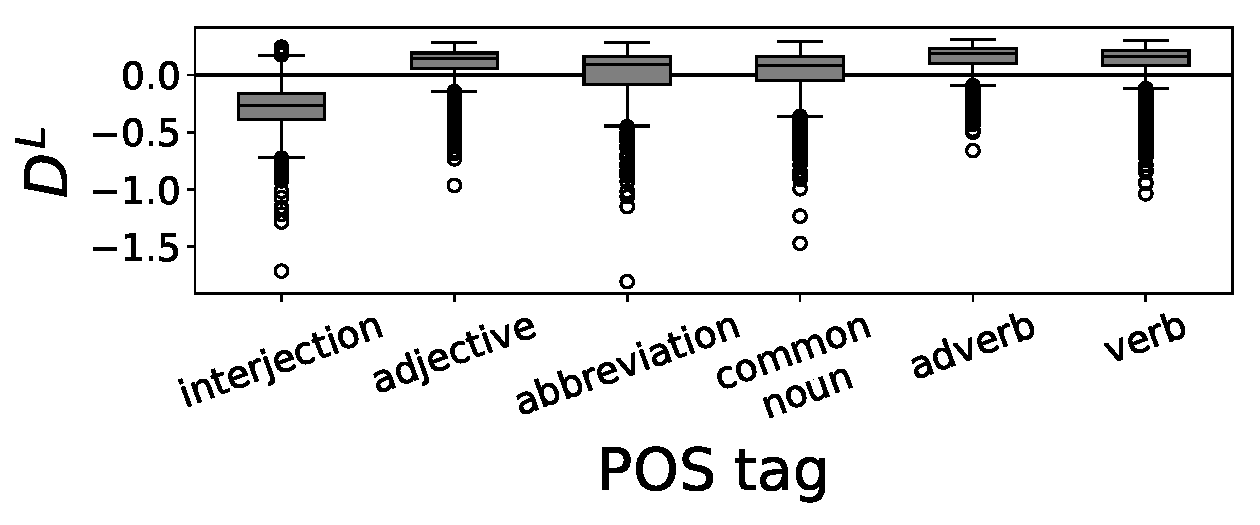
\includegraphics[width=\columnwidth]{figures/pos_DL_distribution.pdf}
\caption{Distribution of mean linguistic dissemination ($D^{L}$) across part of speech groups.}
\label{fig:pos-cd-dist}
\end{figure}

\paragraph{Grammatical aspects of linguistic dissemination}

To confirm the grammatical aspects captured by linguistic dissemination, we visualize the distribution of $D^{L}$ values across words grouped by part of speech tags.
%The grammatical aspects of linguistic linguistic dissemination are confirmed with the distribution of $D^{L}$ across part of speech tags. 
These tags were obtained automatically from the CMU Twitter Part-of-Speech tagger~\cite{gimpel2011}.\footnote{\url{https://github.com/brendano/ark-tweet-nlp} (Accessed 17 June 2017).}
As shown in \autoref{fig:pos-cd-dist}, interjections have lower linguistic dissemination, which follows from being restricted to sentence-initial or sentence-final position. 
In contrast, adjectives and adverbs have high linguistic dissemination because they can appear throughout the sentence, often near open-class words such as nouns and verbs. 
But while these differences are real and in some cases substantial (one-way ANOVA between part-of-speech groups: $F=822.6, p < 0.0001$), robustness checks in ~\autoref{sec:results-binary-predict} show that the role of linguistic dissemination in explaining word growth goes beyond part-of-speech category.

\paragraph{Success prediction: robustness checks}

Considering the uneven distribution of linguistic dissemination across part-of-speech groups (see ~\autoref{fig:pos-cd-dist}), the prediction results may be explained by an imbalance of POS tags between the growth and decline words.
This issue is addressed through two robustness checks: within-group comparison and prediction.

\begin{figure}
\centering
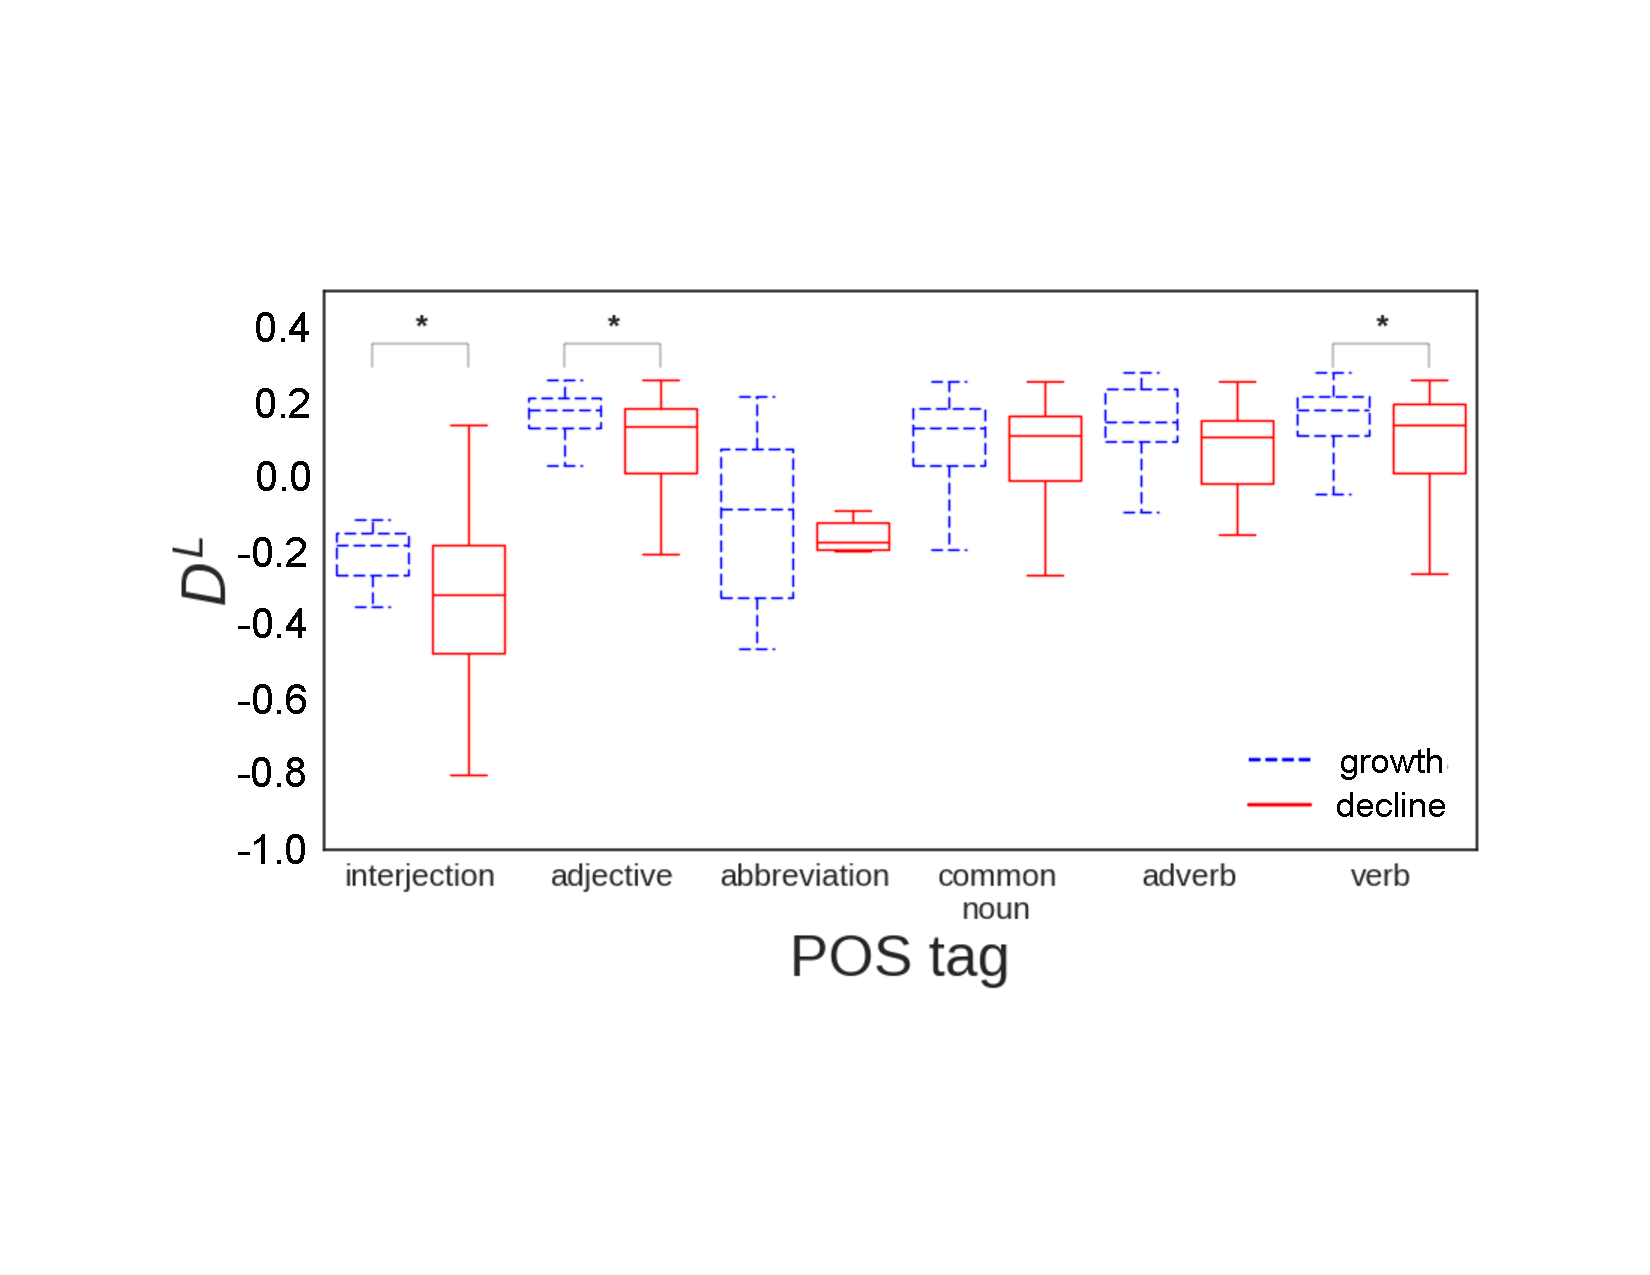
\includegraphics[width=\columnwidth]{figures/growth_vs_decline_matched_pos_DL_distribution_1_12.pdf}
% generated with scripts/frequency/plot_success_vs_failure_pos_DL_distribution.sh
\caption{Distribution of $D^{L}$ values across growth and decline words, grouped by part of speech tag. 
* indicates $p<0.05$ in one-tailed t-test between growth and decline $D^{L}$ values.}
\label{fig:success_vs_failure_pos_DL_distribution}
\end{figure}

First, we compare the distribution of linguistic dissemination values between growth and decline words, grouped by the most common POS tags.
Each decline word is matched with a growth word based on similar mean frequency in the first $k=12$ months, and their mean linguistic dissemination values during that time period are compared, grouped within POS tag groups.
The differences in~\autoref{fig:success_vs_failure_pos_DL_distribution} show that across all POS tags, the growth words show a tendency toward higher linguistic dissemination with significant ($p<0.05$) differences in the interjections and verbs.

Next, the POS tags are used in the same binary prediction task as before, in two different models: (1) as sole features, (2) as additional features in the frequency-only model, each with one month of data ($k=1$).
The linguistic dissemination model significantly outperforms both models (mean accuracy of 50.6\% and 54.8\% respectively), which suggests that the difference in linguistic dissemination between the growth and decline words is not explained by a difference in the POS distribution.

%\begin{figure*}[t!]
%\centering
%\begin{subfigure}[t]{\textwidth}
%\includegraphics[width=\textwidth]{figures/growth_best_fit.pdf}
%\caption{}
%\label{fig:example_time_series_growth}
%\end{subfigure}
%\begin{subfigure}[t]{\textwidth}
%\includegraphics[width=\textwidth]{figures/logistic_decline_best_fit.pdf}
%\caption{}
%\label{fig:example_time_series_decline_logistic}
%\end{subfigure}
%\begin{subfigure}[t]{\textwidth}
%\includegraphics[width=\textwidth]{figures/piecewise_decline_best_fit.pdf}
%\caption{}
%\label{fig:example_time_series_decline_piecewise}
%\end{subfigure}
%\caption{Frequency time series for words from the (a) growth, (b) logistic decline and (c) piecewise decline word sets.}
%\label{fig:example_time_series}
%\end{figure*}
%
%The growth and decline trajectories of the best-fitting words from each word set ($\mathcal{G}, \mathcal{D}_{l}, \mathcal{D}_{p}$; from~\autoref{tab:example_growth_decline_words}) are shown in~\autoref{fig:example_time_series}. 
%The growth words (a) have a clear monotonic growth trajectory, and the decline words (b,c) all follow a similar trajectory of growth up to a peak followed by gradual decline.

\end{appendices}